\chapter*{开题报告}

\setcounter{chapter}{1}

\section{研究工作的背景与意义}
\subsection{研究背景}

随着信息技术产业的高速发展,数字信息量呈爆炸式增长。Gartner研究表明\citing{gartner2015} ,仅2015年的移动数据流量就较2014年增长59\%;并且,这一增长率将持至2018年末,移动数据流量水平达1.73亿TB。数据的快速增长导致企业面临的存储和管理成本越来越高\citing{敖莉2010重复数据删除技术}。另一方面,在存储系统所保存的数据中,高达60\%的数据都是冗余的,随着时间的推移,这些冗余数据的比例将进一步上升\citing{mcknight2006digital}。近年来,存储系统中数据高冗余的特点得到越来越多研究人员的关注,利用该特点来节省存储容量是一个热门研究课题。

数据重删技术(data deduplication)是指通过识别数据流中的冗余,只传输或存储唯一数据(unique data),而使用指向已存储数据的指针替换重复副本, 以达到节省带宽或存储空间的目的\citing{2012重复数据删除关键技术研究进展}。由于能够有效地降低存储开销,数据重删技术非常适合为管理日益增长的海量数据节省成本。在工业界,EMC Data Domain\citing{EMCDataDomain}和Avamar\citing{Avamar}、Veritas的NetBackup Appliances\citing{veritas} 以及Commvault的开放数据平台\citing{CommVault} 都是比较知名的数据重删应用产品;此外,各大云存储厂商(例如 Dropbox、Google Drive、Bitcasa、Moza等)也纷纷将数据重删技术应用于各自的云服务产品中,以提升经济效益\citing{harnik2010side}。

如图\ref{fig:数据重删系统的存储模式}所示,在支持数据重删的存储系统(统称为数据重删系统)中,重删后的任何数据块都被一个或多个文件引用,而文件则以指向这些数据块的指针的集合形式存储。这种文件共用数据块的存储模式强调了数据块的敏感性,因为一个数据块的泄漏可能扩散影响到共用这个数据块的所有文件。如何保护重删后的数据的隐私,成为信息安全领域的一个研究热点。

\begin{figure}[!htb]
    \small
    \centering
    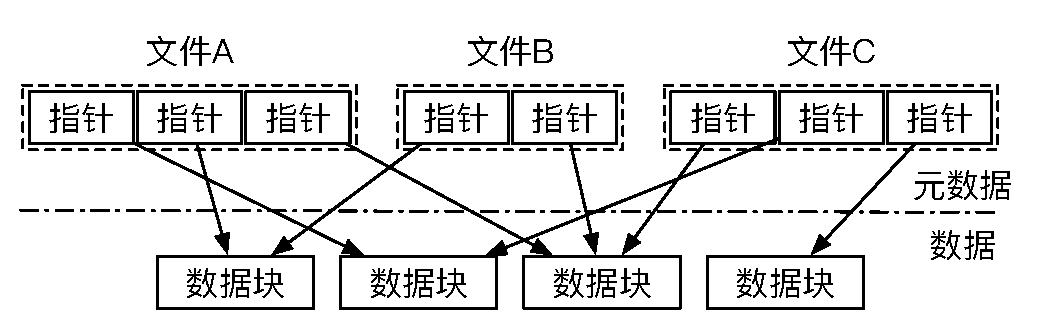
\includegraphics[width=10cm]{DedupSystemStorageMode}
    \caption{数据重删系统的存储模式} 
    \label{fig:数据重删系统的存储模式}
\end{figure}

为了保护数据隐私,加密重复数据删除(encrypted deduplication)增加了一层作用于逻辑数据块的加密操作。如图\ref{fig:加密重复数据删除系统逻辑视图}所示,该加密层基于数据内容来产生加密密钥\citing{bellare2013message}(例如将数据块的哈希值作为密钥\citing{douceur2002reclaiming}),从而将相同的明文数据块加密为相同的密文数据块。系统计算每个密文数据块的哈希值(称为指纹,fingerprint),查询指纹索引(fingerprint index)确定该数据块是否已经存储,最后保存仅具有唯一指纹的密文数据块。需要指出的是,部分加密重复数据删除方案\citing{bellare2013message}采用随机加密算法,但基于明文数据块产生指纹,因此仍然可以通过检查指纹来识别重复数据。

\begin{figure}[!htb]
    \small
    \centering
    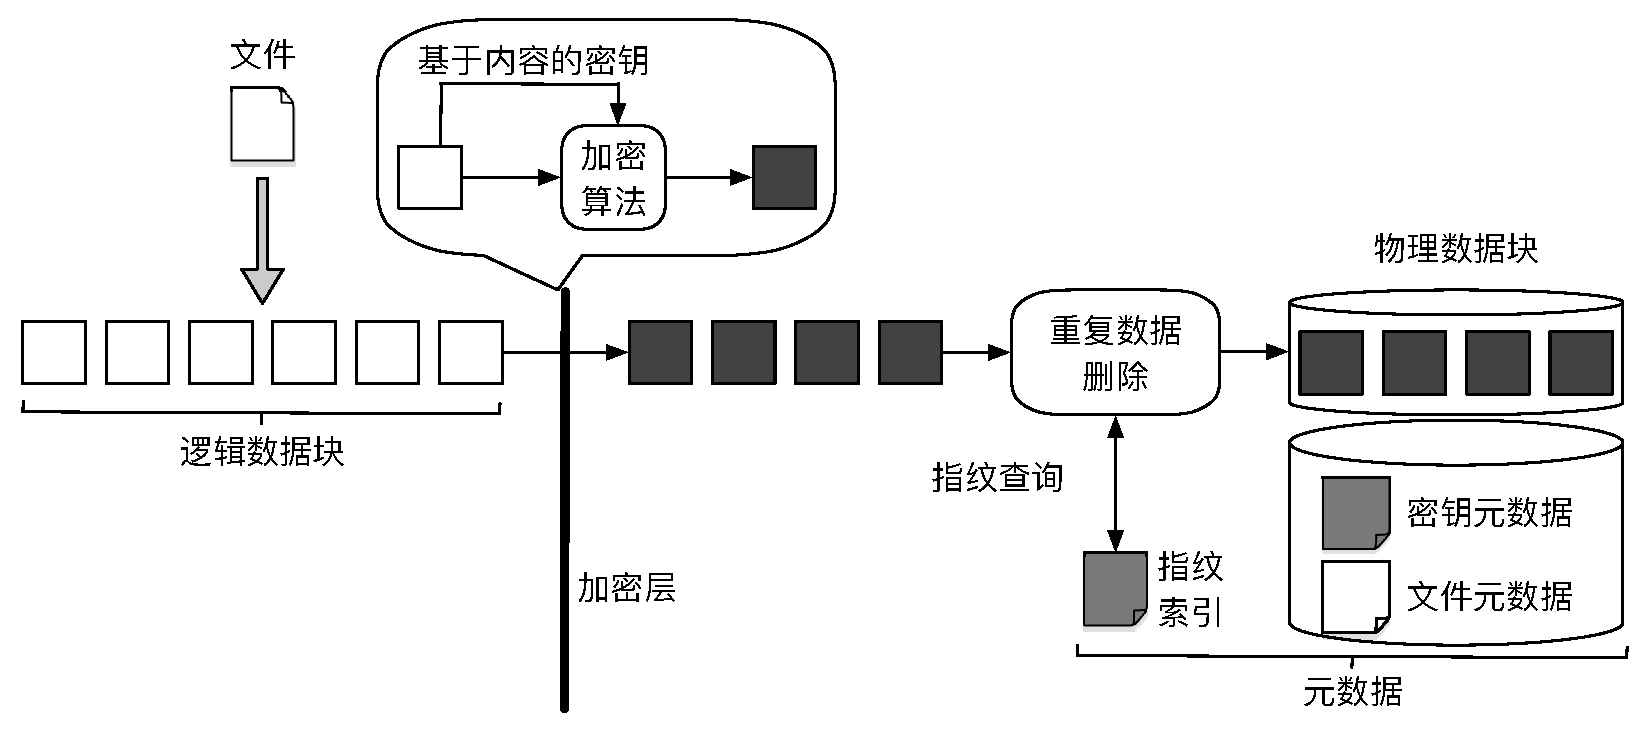
\includegraphics[width=14cm]{EncryptDedupSystemLogic}
    \caption{加密重复数据删除系统逻辑视图}
    \label{fig:加密重复数据删除系统逻辑视图}
\end{figure}

除了指纹索引以外,加密重复数据删除系统须存储额外的元数据(metadata),包括:
\begin{enumerate}
    \item 文件元数据记录了文件内逻辑数据块与相应物理数据块的映射关系,用于重构完整文件。
    \item 密钥元数据记录了文件内逻辑数据块的解密密钥,用于恢复相应的明文内容,由于密钥元数据包含密钥信息,需由文件属主的主密钥(master key)加密后以密文形式存储。
\end{enumerate}

\subsection{问题和动机}

\textbf{密钥生成的安全性和效率平衡问题}

%TODO:数据块信息引用
由于基于数据块内容产生密钥,加密重复数据删除泄漏了数据块的频率信息,即如果一个明文数据块出现了n次,则它对应的密文数据块也将出现n次。另一方面,真实数据集中数据块的出现频率往往呈非均匀分布,调研了FSL和VM备份数据集的数据块频率分布特征,发现三种数据集有超过97\%的数据块的频率低于100次,而至多只有0.04\%的数据块的频率高于10,000次(图\ref{fig:两种真实数据集的数据块频率分布}),这种非均匀的分布特点使攻击者可以利用频率来确定相应数据块。

基于以上原因,认为加密重复数据删除可能受到频率分析\citing{naveed2015inference}的威胁,拟通过本课题,深入研究频率分析攻击对加密重复数据删除安全性的影响,以及提高频率分析攻击效果的方法。

\textbf{重复数据删除中的安全性和效率平衡问题}

从\ S \ ref {sec:introduction}中回想起,现有的加密重复数据删除实现需要昂贵的密码保护。 服务器辅助的MLE必须使用OPRF协议\ cite {naor04}来保护指纹信息免受密钥服务器的侵害,但是OPRF协议涉及昂贵的公钥加密操作(请参见\ S \ ref {subsec:synthetic}中的Exp \#1 )。 同样,当前的PoW实现基于Merkle树协议\ cite {halevi11},该协议对块级PoW执行许多哈希计算。 尽管我们可以通过在每个文件的基础上应用PoW来减轻PoW的计算量(即客户端证明其拥有文件所有权),但是云无法在基于块的重复数据删除下验证块是否属于文件。 现有的提高服务器辅助MLE或PoW性能的解决方案通常会牺牲安全性\ cite {li20b,xu13,pietro12},带宽效率\ cite {harnik10,li15}或存储效率\ cite {zhou15,qin17,li20b}(\ S \ ref {sec:related_work})。


\subsection{研究意义}

本课题研究将填补频率分析攻击研究空白,对理解加密重复数据删除的实际安全性,并降低其在非适合场景下的误用风险具有重要作用。

尽管加密重复数据删除的频率泄漏已是学术界公认的安全问题,但针对性的频率分析攻击研究仍为空白(即利用频率泄漏来获取隐私数据仍是一个开放性问题),致使部分厂商盲目地将加密重复数据删除技术应用于商业产品\citing{MEGA,ElephantDrive}和开源系统\citing{Cryptosphere,Freenet,GNUP2P,Tahoe-LAFS}中。本项目将研究加密重复数据删除技术在频率分析攻击下的实际安全性,以指导其在适合场景下被正确使用。


\section{国内外研究历史与现状}

\subsection{加密重复数据删除}
\label{sec:加密重复数据删除}
在传统对称加密方式下,每个用户具有不同的密钥,不同用户之间的相同明文会被加密为不同密文,难以执行(密文)重复数据删除操作。

消息锁定加密(message-locked encryption,MLE)确立了加密重复数据删除的密码学基础\citing{bellare2013message}:基于数据内容产生密钥(称为 MLE 密钥),从而将相同明文加密为相同密文。最流行的MLE实例是收敛加密(convergent encryption,CE)\citing{douceur2002reclaiming},它使用明文的哈希值作为MLE密钥,并基于密文哈希值计算指纹,以识别重复数据(如图\ref{fig:加密重复数据删除系统逻辑视图})。基于CE的加密重复数据删除方案还包括:

\begin{enumerate}
    \item 哈希收敛加密(hash convergent encryption,HCE)\citing{douceur2002reclaiming}与CE具有相同的MLE密钥产生规则,但基于明文哈希值计算指纹。
    \item 随机收敛加密(random convergent encryption,RCE)\citing{douceur2002reclaiming}使用随机密钥加密以产生非确定的密文,同时也基于明文哈希值来进行重复检查。
    \item 收敛扩散(convergent dispersal,CD)\citing{li2016cdstore}使用明文哈希值作为秘密共享(secret sharing)的输入种子,在兼容重复数据删除的基础上 提高了密文存储的可靠性。
\end{enumerate}

上述MLE实例基于明文产生MLE密钥(CE、HCE和CD)或指纹(HCE和RCE),如果明文是可预测的(即所有可能的明文的数量有限),这些方案易于受到离线暴力破解攻击\citing{bellare2013message,keelveedhi2013dupless}。为了抵御该攻击,DupLESS\citing{keelveedhi2013dupless}基于第三方密钥服务器实现了服务器辅助 MLE(server-aided MLE),确保无法从离线明文派生出相应的MLE密钥。以服务器辅助MLE为基础,现有研究进一步解决了加密重复数据删除的故障容错\citing{li2015cdstore,duan2014distributed}、透明价格模型\citing{armknecht2015transparent}、点对点密钥管理\citing{liu2015secure}、层次密钥管理\citing{zhou2015secdep}等问题。围绕MLE扩展功能的一系列研究包括:兼容加密重复数据删除的数据完整性审计协议\citing{li2016secure};支持动态访问控制的加密重复数据删除系统REED\citing{li2016rekeying,qin2017design}。

无论是MLE还是服务器辅助MLE,均须为相同的明文产生相同的密文(CE、HCE、CD和DupLESS)或指纹(HCE和RCE),泄漏了数据的出现频率。一些理论研究\citing{abadi2013message,stanek2014secure,bellare2015interactive}基于零知识证明、全同态加密、双线性对运算等底层密码技术实现了随机加密,但这些方案存在计算复杂性高、依赖多轮信息交互等问题,难以应用到系统实践中。本文关注可实际应用的加密重复数据删除系统/方案的频率泄漏问题,研究其安全性影响和防御对策。

\subsection{数据所有权证明}
\label{sec:数据所有权证明}

Source-based deduplication is bandwidth-efficient but vulnerable to
side-channel attacks \cite{harnik10} (\S\ref{subsec:encrypted-dedup}). 
Prior studies \cite{harnik10, li15} combine source-based deduplication and
target-based deduplication to defend against side-channel attacks, while
\sysname achieves
significantly more bandwidth savings by purely performing source-based
deduplication (\S\ref{subsec:real-world}) and using PoW to protect against
side-channel attacks.  Also, \sysname is much more efficient than
Merkle-tree-based PoW (\S\ref{subsec:synthetic}).  Some other studies make PoW
efficient by relaxing security (e.g., \cite{pietro12,xu13}), while \sysname
uses client-side SGX to preserve the security of PoW.

\subsection{基于SGX的存储系统}
\label{sec:基于SGX的存储系统}

SGX \cite{sgx} has been widely used for
securing storage systems.  PESOS \cite{krahn18}  enforces the access policies
of object storage with SGX.  OBLIVIATE
\cite{ahmad18} enhances the security of SGX-based file systems against
privileged side-channel attacks. EnclaveDB \cite{priebe18} and ObliDB
\cite{eskandarian19} protect outsourced databases against information leakage
via SGX.  NEXUS \cite{djoko19} enables fine-grained access control with SGX
over untrusted cloud storage.
On the performance side, Harnik {\em et al.} \cite{harnik18} propose
guidelines on mitigating the performance overhead of SGX implementations.
ShieldStore \cite{kim19} implements application-specific
data management to limit the enclave memory usage.  SPEICHER \cite{bailleu19}
is an SGX-based LSM-based key-value store with efficient I/O operations.  

% to address the I/O performance bottleneck
% of enclave.

All the above studies do not consider deduplication. Dang {\em et al.}
\cite{dang17} propose proxy-based protocols for bandwidth-efficient encrypted
deduplication, but the protocols do not address the key generation performance
overhead and have no implementation. SPEED \cite{cui19} leverages deduplication
to make SGX computations efficient, but \sysname improves the performance of
encrypted deduplication with SGX.  SeGShare \cite{fuhry20} maintains a
cloud-side enclave for secure file-based deduplication, while \sysname uses a
client-side enclave to implement an efficient PoW protocol and supports more
fine-grained chunk-based deduplication. 


\section{课题的研究内容、研究目标、以及拟解决的关键问题}
\subsection{研究内容}

% \subsubsection*{加密重复数据删除的频率分析攻击}

% 在传统频率分析模式下,攻击者能够访问明文逻辑数据块集合M和密文逻辑数据块集合$C$($M$和$C$包含重复的明文和密文数据块)。攻击者根据出现频率分别对$M$和$C$中的数据块进行排序,然后将$C$中的密文数据块映射为$M$中与其具有相同排名的明文数据块。但是,传统频率分析在加密重复数据删除中难以形成有效的攻击,主要原因是:$M$和$C$的原始内容可能存在差异(例如$M$和$C$来源于同一个文件系统在不同时间点的备份镜像),将打乱数据块频率排序的对应关系;并且,在频率排序过程中可能存在大量明文和密文数据块具有相同的频率,频率分析难以排序这些数据块来形成正确的对应关系。

% 为了提高传统频率分析的攻击效果,首先研究基于数据特征的新型频率分析攻击技术。然后,分别从抵抗频率排序干扰和降低攻击发生条件两方面改进攻击技术。最后,实现针对真实系统的频率分析攻击原型,并分析该攻击对各类数据安全性的影响。


\subsection{研究目标}

针对以上研究内容,预期实现如下研究目标: 
\begin{enumerate}
    \item 在理论上,设计基于可信计算硬件的密钥生成和数据块所有权证明机制,并在相应安全假设下论证其安全性。
    \item 在技术上,以理论研究为支撑,设计并实现符合安全性假设的低开销的服务器辅助密钥生成和安全且高效的重复数据删除,设并在真实系统中进行理论验证和攻击效果测试。 
\end{enumerate}


\subsection{拟解决的关键问题}

本课题致力于解决传统服务器辅助密钥生成机制和客户端重复数据删除场景下的数据块所有权证明机制的效率问题,难以解决的如下问题:

\begin{enumerate}
    \item How should enclaves be managed?
    \begin{itemize}
        \item Enclave startup incurs high overhead due to remote attestation
        \item Key enclave needs to manage system wide secret information κ
        \item Client machine cannot persistently maintain enclaves
    \end{itemize}
    \item How does key manager prevent online brute force attack?
    \begin{itemize}
        \item Need to enable revocation on clients’ querying key generation oracle
    \end{itemize}
    \item How can key generation performance be further improved?
    \begin{itemize}
        \item Expensive overhead in establishing secure channel (taking ~70\% overallkeygen overhead)
    \end{itemize}
\end{enumerate}


    


    


\section{拟采取的研究方案}
\label{sec:技术路线}



如图\ref{fig:技术路线图}所示,在支撑研究(基于数据块局部性的频率分析攻击方案\citing{li2017information})的基础上,根据相对频率分布特性,设计抗排序干扰的攻击方法;在数据相似性的基础上,设计低依赖条件的攻击方法。最终设计出针对加密重复数据删除方案/系统的新型频率分析攻击方法及对应的原型软件工具。

\begin{figure}[!htb]
    \small
    \centering
    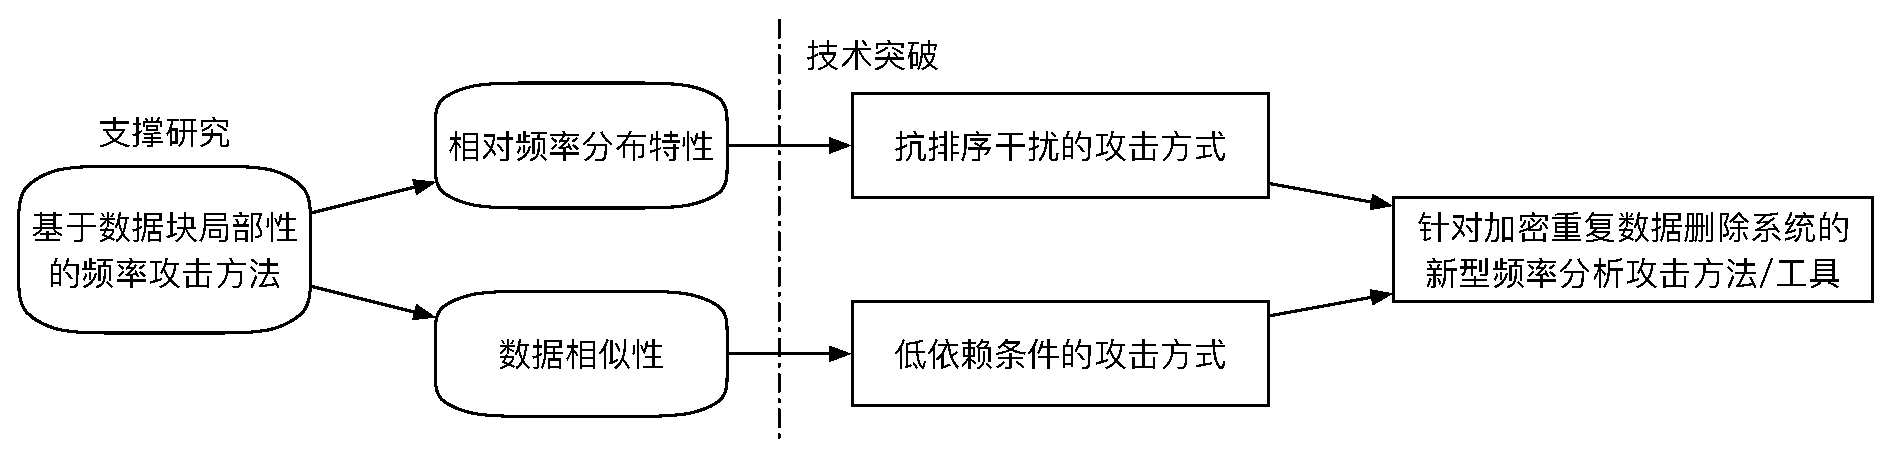
\includegraphics[width=15cm]{TechnicalRoute.eps}
    \caption{技术路线图} 
    \label{fig:技术路线图}
\end{figure}

\subsection{支撑研究}

% 基于数据块局部性的频率分析攻击方案(locality-based attack)\citing{li2017information}作为支撑研究,该方案主要用于破译加密数据备份,即已知的明文数据块集合$M$和目标密文数据块集合$C$源于同一个系统在两个不同时间点的备份镜像。攻击利用了数据块的局部性特征:在不同备份之间,绝大多数数据块保持了相同的局部顺序;例如,每天备份工作项目的进度快照,若一天内的改动较小,则在两次备份之间未被改动的大部分数据块之间的相对顺序保持不变。因此,得出一个关键推论:如果明文数据块M是密文数据块$C$的原始明文,那么M左边和右边相邻的明文数据块有较大可能也是$C$左边和右边相邻密文数据块的原始明文。

% \begin{figure}[!htb]
%     \small
%     \centering
%     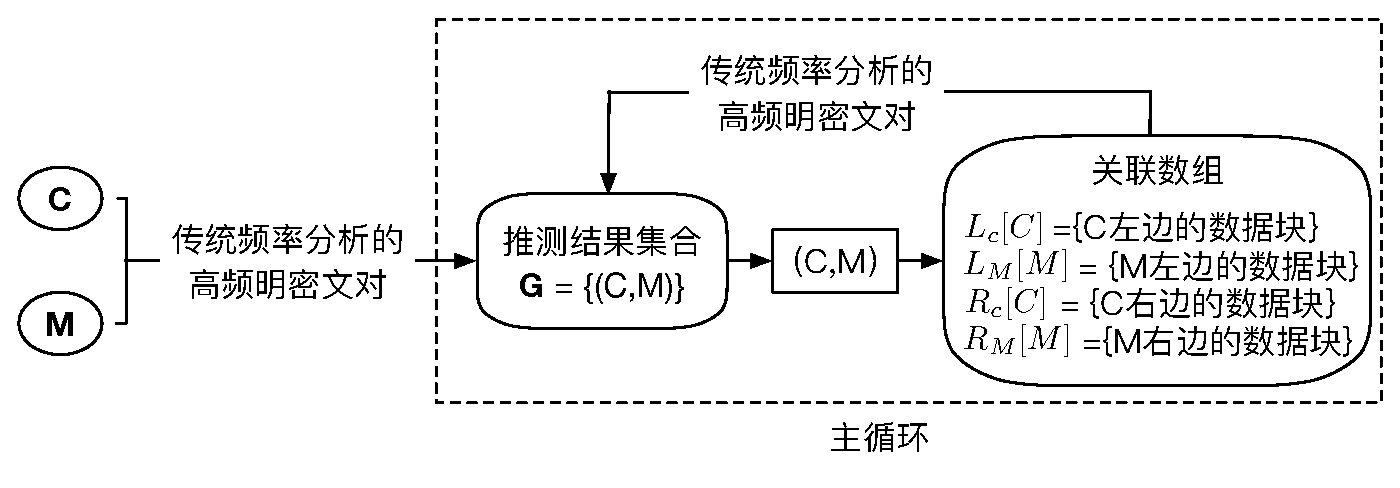
\includegraphics[width=14cm]{BaseFrequencyAttack}
%     \caption{基于数据块局部性的频率分析攻击} 
%     \label{fig:基于数据块局部性的频率分析攻击}
% \end{figure}


% 基于此,攻击流程如图\ref{fig:基于数据块局部性的频率分析攻击}所示:首先,对$C$和$M$应用传统频率分析(\ref{sec:传统频率分析攻击}),将获得的若干组高频明密文对加入推测结果集合 $G$;然后,每次从$G$中选取一组明密文对$(M,C)$,分别对其左右相邻的明文和密文数据块集合$L_M[M]$和$L_C[C]$,以及$R_M[M]$和$R_C[C]$实施频率分析,并将获得的高频明密文对也加入$G$;继续对$G$中的明密文对进行基于相邻数据块的频率分析,直至所有明密文对都被处理。

% 为了验证攻击效果,定义推测率为正确推测出原始明文的(不同)密文数据块个数与$C$中(不同)密文数据块总个数的比率。在基于真实数据集的实验验证中,攻击方案能够达到17.8\%推测率,远远高于传统频率分析方法的0.0001\%推测率。


% \subsection{技术突破}

% \subsubsection{基于分布的频率分析攻击方法}


% \par 基于分布的频率分析攻击利用密文和明文的相对顺序信息来增强频率分析的有效性。该攻击方法建立在数据块局部性\citing{xia2011silo,lillibridge2009sparse,zhu2008avoiding}的基础上。通过以下三个关键特性构造出基于分布的频率分析攻击方法。

% \begin{itemize}
%     \item 数据块局部性指出数据的原始排序可能会在各种备份文件中得以保留,因此可以用于在备份文件中推理出类似的与位置相关的密文-明文对。
%     \item 相邻数据的共现频率的相对频率分布可以通过分析得到。
%     \item 明文及其相应的密文具有相似的相对频率分布的特性。
% \end{itemize}
 
% \subsubsection{基于聚类的频率分析攻击方法}


% 在基于分布的频率分析攻击方法的基础上,通过引入相似性\citing{bhagwat2009extreme}这一属性来消除基于分布的频率分析攻击方法对明文数据的细粒度顺序信息的需求。基于此提出基于聚类的频率分析攻击方法。

\section{可行性分析}

\subsection{研究方法可行}

本课题通过引入加密重复数据删除方案/系统的相关特性来设计新型频率分析攻击方法,针对性提高频率分析攻击方法的有效性。该研究问题具有很高的实际价值且在面向加密重复数据删除的攻击中,已有工作提出了基于数据块局部性(chunk locality)\citing{zhu2008avoiding,lillibridge2009sparse,xia2011silo}的频率分析攻击\citing{li2017information},在此基础上改进攻击方案以提高频率分析攻击实际效果具有明确的可行性。

\subsection{研究条件可行}

前期基于数据块局部性的频率分析攻击方案给出了本课题研究两种新型频率分析攻击方法的基本理论和工具基础。在原有方案上改进即可用于本课题研究。研究者在本科阶段深入钻研了CDStore、REED、SDFS等加密重复数据删除系统,以及前期基于数据块局部性的频率分析攻击方案的理论和工具实现。这些经验可以帮助设计新型频率分析方法以及其在真实系统中的实践。

\section{本研究特色与创新之处}

本研究的特色与创新之处有以下几点:

% \begin{enumerate}
%     \item 研究针对加密重复数据删除提出了两种新型的频率分析攻击方法。除了利用由于加密重复数据删除具有确定性导致的频率泄漏之外,两种攻击都利用重复数据删除工作负载的特性来增加频率分析攻击的有效性。
%     \item 本文研究使用多个真实数据集(包括长期备份\citing{sun2016long,FSL14},Windows文件系统快照\citing{meyer2012study}和VM磁盘映像\citing{li2016cdstore,qin2017design})以及开源重复数据删除系统SDFS\citing{SDFS}、Destor\citing{Destor},评估两种新型频率分析攻击方法和基本频率分析攻击方法的实际效果。通过评估频率攻击方法的攻击结果,进一步分析本频率分析攻击方法对实际加密重复数据删除带来的安全性影响。
%     \item 本研究讨论了减少加密重复数据删除中信息泄漏的可能方案。
% \end{enumerate}

We propose \sysname, a high-performance SGX-based encrypted deduplication
system. \sysname builds on server-aided MLE as in DupLESS \cite{bellare13b},
but executes efficient OPRF-less MLE key generation and PoW inside enclaves.
In particular, it comprises three major building blocks:
%
\begin{itemize}[leftmargin=*] 
\item 
{\em Secure and efficient enclave management}: It protects against the
compromise of the key server and allows a client to quickly bootstrap an
enclave after a restart.
\item 
{\em Renewable blinded key management}: It generates a blinded key for
protecting the communication between the enclave inside the key server and
each of the clients based on key regression \cite{fu06}, such that the blinded
key is renewable for dynamic client authentication. 
\item 
{\em SGX-based speculative encryption}:  It offloads the online
encryption/decryption overhead of an enclave via speculative encryption
\cite{eduardo19}. 
\end{itemize}